\documentclass[10pt,leqno]{beamer}
\usepackage{amsmath,amsfonts}	% use math symbols
\usepackage{graphicx} % insert images
\usepackage{url} % insert urls
\usepackage{hyperref}
\usepackage{amsthm}
\usepackage{auto-pst-pdf}
\setbeamertemplate{navigation symbols}{}
\usepackage{listings}
\usepackage{xcolor}
\usepackage{moresize}

\definecolor{cream}{rgb}{1.0, 0.99, 0.82}

\lstset{frame=single, basicstyle=\color{black}\ttfamily\ssmall, backgroundcolor=\color{cream}}



%%%%%%%%%%%%%%%%%%%%%%%%%%%%%%%%%%%%%%%%%%%%



\begin{document}

\title{A Brief Introduction to the Command Line}
\author{Hautahi Kingi}
\date{}


\maketitle
%%%%%%%%%%%%%%%%%%%%%%%%%%%%%%%%%%%%
\begin{frame}[fragile]{Introduction}

A \textbf{shell} is a computer program like any other. But its primary purpose is to read commands and run other programs, rather than to perform tasks/calculations itself.\\~\\


We interact with the shell through a command-line interface or \textbf{terminal}. We do so by entering commands as text input. The terminal reads the text input, interprets the commands and sends instructions to the shell, which then executes the appropriate operating system functions. Once the commands are carried out, the shell communicates this with the terminal which then prints its output.

\end{frame}


%%%%%%%%%%%%%%%%%%%%%%%%%%%%%%%%%%%%
\begin{frame}[fragile]{Getting Started}

Type \emph{whoami} into the terminal.
\begin{lstlisting}
$ whoami
hautahikingi
$ 
\end{lstlisting}
The command's output is the ID of the current user. When we type \emph{whoami}, the shell finds a program called whoami, runs that program, displays that program's output (your username), then displays a new prompt to tell us that it is ready for more commands.\\~\\

Now let's try the following.
\begin{lstlisting}
$ pwd
/Users/hautahikingi
\end{lstlisting}
This stands for \emph{print working directory}. When you first login, your current working directory is your home directory.


\end{frame}

%%%%%%%%%%%%%%%%%%%%%%%%%%%%%%%%%%%%
\begin{frame}[fragile]{Exploring a Directory}

To find out what is in your home directory, type
\begin{lstlisting}
$ ls				
Desktop		Dropbox		Pictures	Documents	essay.txt	Downloads	Movies
\end{lstlisting}
\emph{ls} prints the names of the files and directories in the current directory in alphabetical order, arranged neatly into columns.\\~\\

A number of commands have extra options or features which we can call through the use of a \textbf{flag}.
\begin{lstlisting}[frame=single]
$: ls -l
total 8
drwx------+  53 hautahikingi  staff   1802 Jul 21 22:34 Desktop
drwxr-xr-x+  21 hautahikingi  staff    714 Jul  8 13:25 Documents
drwx------+ 503 hautahikingi  staff  17102 Aug  5 11:07 Downloads
\vdots
\end{lstlisting}
The -l flag on the \emph{ls} command is short for long format and it displays a more detailed listing of the files within the current working directory, including file size and date last modified. Note that there is a space between ls and -l: without it, the shell thinks we're trying to run a command called ls-l, which doesn't exist.\\~\\

Try the -F flag. What does this do?
\end{frame}

%%%%%%%%%%%%%%%%%%%%%%%%%%%%%%%%%%%%
\begin{frame}[fragile]{File Hierarchy}

\begin{center}
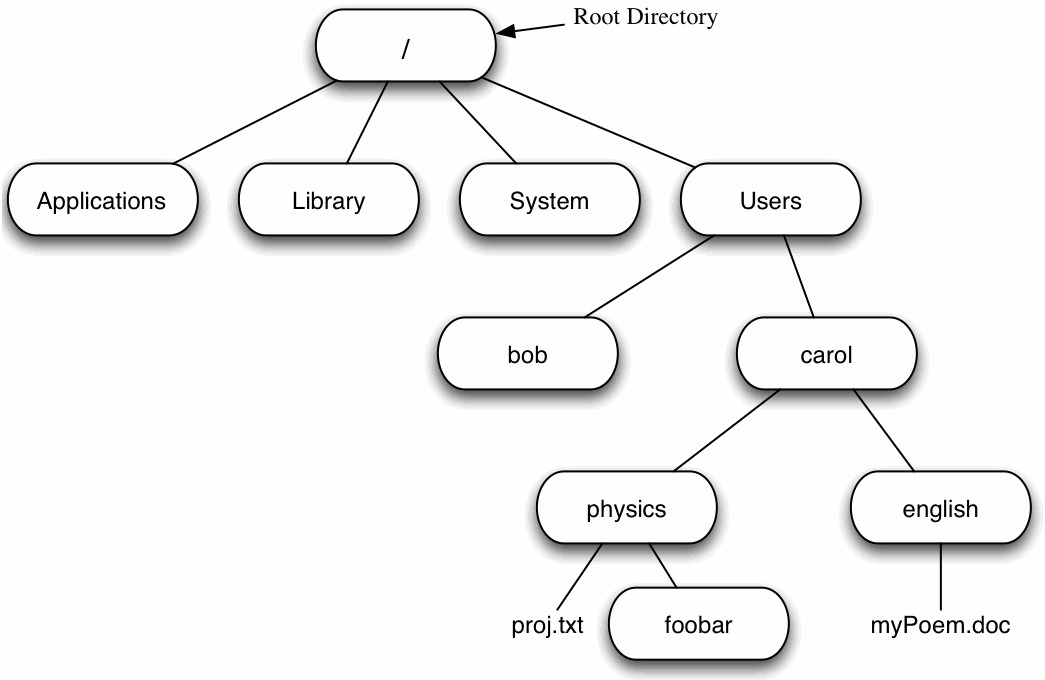
\includegraphics[width=10cm]{./auxfiles/tree.jpg}
\end{center}
The home directory of \emph{carol} contains two sub-directories - \emph{physics} and \emph{english}. The full path to the file \emph{myPoem.doc} is \emph{/Users/carol/english/myPoem.doc}. Notice the two meanings for the / character.

\end{frame}

%%%%%%%%%%%%%%%%%%%%%%%%%%%%%%%%%%%%
\begin{frame}[fragile]{File and Directory Navigation}
We can use \emph{cd} followed by a directory name to change our working directory. \emph{cd} stands for \emph{change directory}, which changes the shell's idea of what directory we are in. In the example above, we can type
\begin{lstlisting}
$ cd /users/carol/physics
\end{lstlisting}
\emph{cd} doesn't print anything, but if we run \emph{pwd} after it, we can confirm that the current working directory is \emph{physics}.
\begin{lstlisting}
$ pwd
/users/carol/physics
\end{lstlisting}
If we run \emph{ls} without parameters now, it lists the contents of /users/carol/physics
\begin{lstlisting}
$ ls
proj.txt 	foobar
\end{lstlisting}

\end{frame}

%%%%%%%%%%%%%%%%%%%%%%%%%%%%%%%%%%%%
\begin{frame}[fragile]{File and Directory Navigation}

We do not have to type the full path to the directory.  Instead, we can use \textbf{relative path references}. When \emph{cd} is followed by a folder path that does not begin with the root directory (/), it assumes that you are first referencing the current working directory. In the above example, because we were located in \emph{/users/carol/} we only needed to type 
\begin{lstlisting}
$ cd physics
\end{lstlisting}
We also do not have to type the entire name of a directory. \emph{Tab Completion} is very handy in situations where the filename is long. Pressing tab asks the terminal to guess what you are trying to type. For example, if we are located in /Users/carol/ and type
\begin{lstlisting}
$ cd ph
\end{lstlisting}
and then press tab, the shell automatically completes the \emph{physics} directory name for us. If, however, there was another directory called \emph{philosophy}, the user would need to type \emph{cd phy} before pressing tab.

\end{frame}

%%%%%%%%%%%%%%%%%%%%%%%%%%%%%%%%%%%%
\begin{frame}[fragile]{Creating Directories}

Let's now make a subdirectory called \emph{my\_thesis} in the Dropbox folder.
\begin{lstlisting}
$ cd Dropbox
$ mkdir my_thesis
$ cd my_thesis
$ pwd
/Users/hautahikingi/Dropbox/my_thesis
\end{lstlisting}
Here, I navigated to the Dropbox folder, made the \emph{my\_thesis} directory, and then navigated into the newly created directory. 
\end{frame}

%%%%%%%%%%%%%%%%%%%%%%%%%%%%%%%%%%%%
\begin{frame}[fragile]{Creating files with a text editor}

Let's now create a new file called \emph{introduction.txt} using a text editor.
\begin{lstlisting}
$ nano introduction.txt
\end{lstlisting}
I am using \textbf{Nano} here because it is the default text editor on a Mac and it is very easy to use. The equivalent on a Windows machine would be \textbf{Notepad}. Let's type in a few lines of text.
\begin{center}
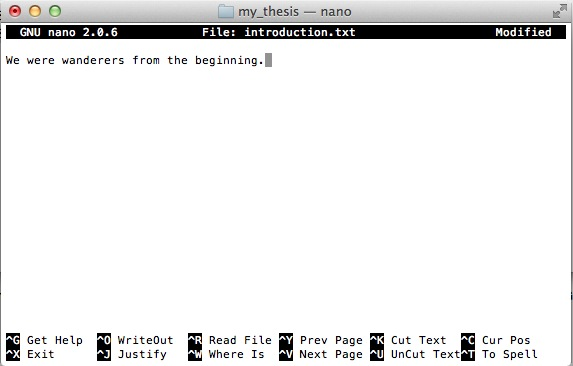
\includegraphics[width=5cm]{./auxfiles/nano.jpg}
\end{center}
In nano, use Control-X to quit the editor and return to the shell. Make sure you save in the process. We can check the changes we've made to a particular file by using the \emph{cat} command.
\begin{lstlisting}
$ cat introduction.txt
We were wanderers from the beginning.
\end{lstlisting}
\end{frame}

%%%%%%%%%%%%%%%%%%%%%%%%%%%%%%%%%%%%
\begin{frame}[fragile]{Command Line/GUI perform the same tasks}
You obviously don't need to create files using the command line. You can do it all the usual way as well. Imagine I just typed up some matlab code which I saved into the my\_thesis folder as \emph{code.m}. Now lets look at:
\begin{lstlisting}
$: ls
code.m	introduction.txt
\end{lstlisting}

\end{frame}


%%%%%%%%%%%%%%%%%%%%%%%%%%%%%%%%%%%%

\setbeamercolor{background canvas}{bg=black}
\begin{frame}[plain]{}



\end{frame}
\setbeamercolor{background canvas}{bg=white}

%%%%%%%%%%%%%%%%%%

\end{document}
